\documentclass[12pt,a4paper]{article}

\usepackage[utf8]{inputenc}
\usepackage[T2A]{fontenc}
\usepackage[russian]{babel}
\usepackage{amsmath,amssymb}
\usepackage{graphicx}
\usepackage{booktabs}
\usepackage{multirow}
\usepackage{geometry}
\usepackage{float}
\usepackage{eso-pic}
\graphicspath{{./}}

\geometry{top=2cm,bottom=2cm,left=2.5cm,right=1.5cm}

\title{\textbf{Лабораторная работа 1.4.5}\\
Изучение колебаний струны}

\author{
    Студент \underline{Шеховцов Василий Максимович}\\
    Группа \underline{Б03-601}\\
    Преподаватель \underline{Ивлев Д.А.}
}

\date{
Московский Физико-технический институт\\
(национальный исследовательский университет)\\
11 ноября 2026 г.
}

\begin{document}

\AddToShipoutPictureFG*{
    \AtPageUpperLeft{
        \hspace{1.5cm}
        \raisebox{-1cm}{
            \makebox[0pt][l]{Шеховцов В.М.}
        }
    }
}

\maketitle

\section{Аннотация}

\textbf{Цель работы:} изучить поперечные стоячие волны на тонкой натянутой струне; измерить собственные частоты колебаний струны и проверить условие образования стоячих волн; измерить скорость распространения поперечных волн на струне и исследовать её зависимость от натяжения струны.

\textbf{Оборудование:} закреплённая на станине стальная струна, набор грузов, электромагнитные датчики, звуковой генератор, двухканальный осциллограф, частотомер.

\section{Теоретические сведения}

Основное свойство струны --- гибкость --- является следствием её большой длины по сравнению с поперечными размерами. Струна практически не сопротивляется изгибу, поэтому изгибные напряжения не учитываются. Сила натяжения $T$ должна значительно превосходить вес струны, чтобы она не провисала.

При малых отклонениях от положения равновесия поперечные колебания струны описываются волновым уравнением
\begin{equation}
    \frac{\partial^2 y}{\partial t^2} = u^2\frac{\partial^2 y}{\partial x^2},
    \label{eq:wave}
\end{equation}
где скорость распространения поперечной волны
\begin{equation}
    u = \sqrt{\frac{T}{\rho_l}},
    \label{eq:u}
\end{equation}
$T$ --- сила натяжения струны, $\rho_l$ --- её погонная плотность (масса на единицу длины). Скорость связана с частотой $\nu$ и длиной волны $\lambda$ соотношением $u = \nu\lambda$.

Для струны длиной $L$ с закреплёнными концами решение уравнения~\eqref{eq:wave} имеет вид стоячей волны $y(x,t)=2a\sin kx\,\sin\omega t$. Концы струны должны быть узлами, откуда следует условие образования стоячих волн: на длине струны укладывается целое число полуволн,
\begin{equation}
    n\,\frac{\lambda_n}{2} = L,\qquad n=1,2,3,\ldots
\end{equation}
Поэтому струна может колебаться лишь на собственных частотах
\begin{equation}
    \nu_n = \frac{u}{2L}\,n = \frac{n}{2L}\sqrt{\frac{T}{\rho_l}}.
    \label{eq:nun}
\end{equation}
Число $n$ равно числу пучностей стоячей волны. Спектр собственных частот определяется длиной, натяжением и погонной плотностью струны и не зависит от модуля Юнга материала.

Колебания поддерживаются вынуждающей силой, поэтому для эффективной раскачки частота генератора должна совпадать с одной из собственных частот (резонанс). Реальные колебания никогда не являются чисто стоячими: из-за потерь энергии при отражении на концах к стоячей волне добавляется малая бегущая компонента, которая переносит энергию вдоль струны и приводит к небольшому <<размытию>> узлов. При слишком большой амплитуде нарушается применимость волнового уравнения (появляются нелинейные эффекты), поэтому возбуждение должно быть слабым.

\section{Экспериментальная установка}

Схема установки приведена на рис.~\ref{fig:setup}. Стальная гитарная струна~1 закреплена горизонтально между стойками~2 и~3 на массивной станине~4. К концу струны, перекинутому через блок, прикреплена платформа с грузами~5, создающими натяжение. Электромагнитный датчик~6, подключённый к звуковому генератору~7, возбуждает колебания струны. Частота измеряется частотомером~10. Колебания регистрирует датчик~8, сигнал с которого подаётся на осциллограф~9.

Возбуждающий датчик располагается вблизи неподвижного конца струны (вблизи узла), регистрирующий --- в пучности. Сила, действующая на струну со стороны датчика, пропорциональна $(B_0+B_\sim)^2\approx B_0^2+2B_0B_\sim$, то есть при $B_\sim\ll B_0$ линейно зависит от тока, а её частота совпадает с частотой генератора.

\begin{figure}[H]
    \centering
    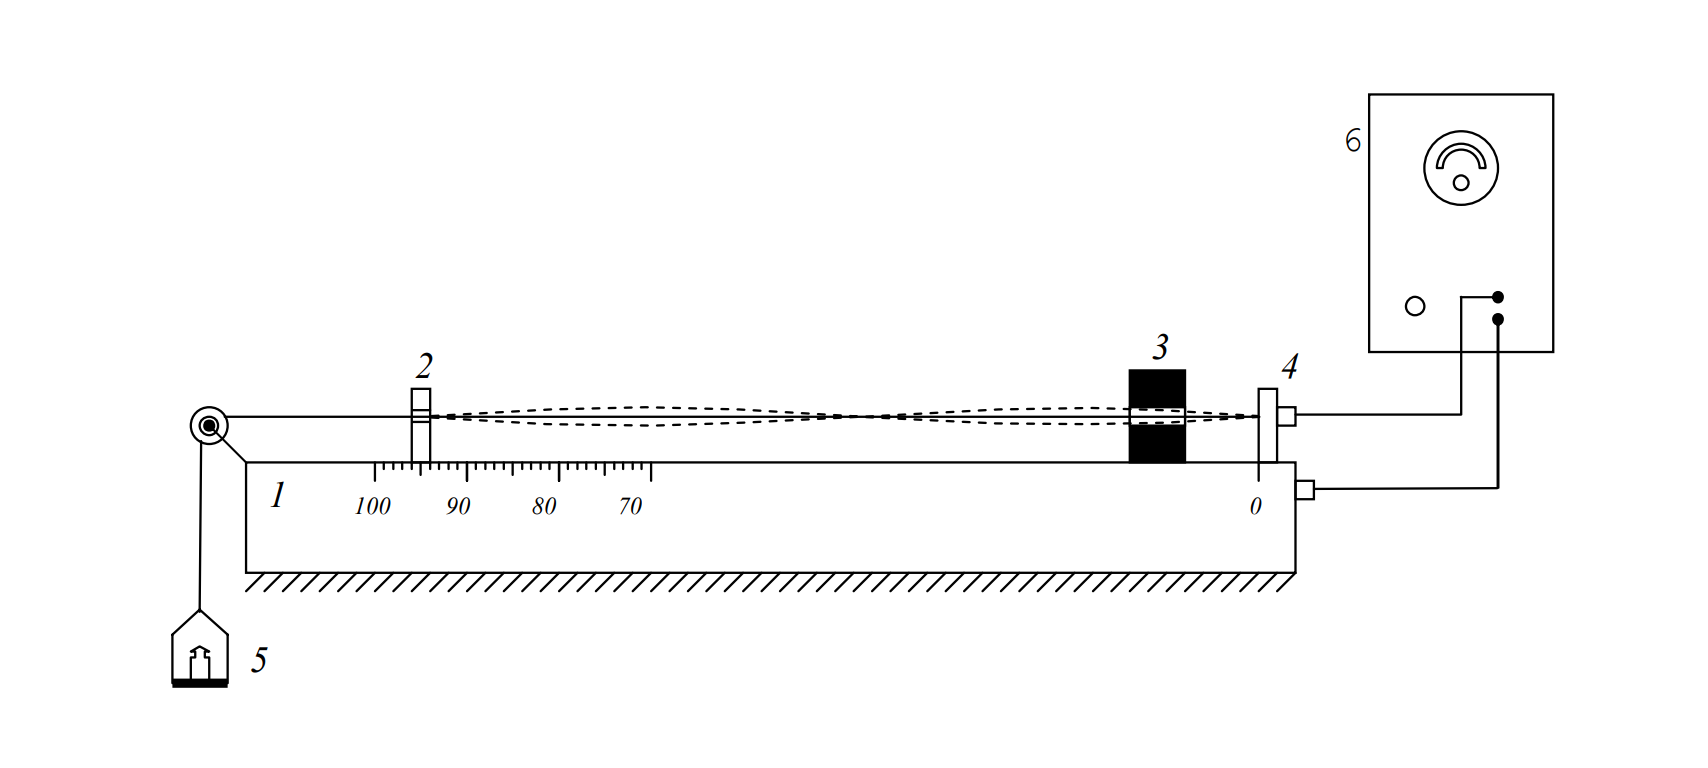
\includegraphics[width=0.85\textwidth]{pic.png}
    \caption{Схема экспериментальной установки}
    \label{fig:setup}
\end{figure}

Длина струны $L = 0{,}500 \pm 0{,}001$~м, табличное значение погонной плотности $\rho_l^{\text{табл}} = 568{,}4$~мг/м $= 5{,}684\cdot10^{-4}$~кг/м.

\section{Обработка результатов}

Резонансные частоты $\nu_n$ измерялись при пяти натяжениях струны. Масса грузов вместе с платформой $m_1=110{,}6+461{,}4+492{,}7=1064{,}7$~г, далее последовательно добавлялись грузы массой $480{,}7$, $500{,}3$, $499{,}1$ и $481{,}7$~г. Сила натяжения $T=mg$, $g=9{,}8$~м/с$^2$

\begin{table}[H]
    \centering
    \caption{Измеренные резонансные частоты $\nu_n$, Гц}
    \begin{tabular}{ccccccccc}
        \toprule
        $m$, г & $T$, Н & $\nu_1$ & $\nu_2$ & $\nu_3$ & $\nu_4$ & $\nu_5$ & $\nu_6$ & $\nu_7$ \\
        \midrule
        1064,7 & 10,445 & 135,3 & 271,6 & 402,1 & 542,2 & 677,0 & 812,9 & 948,9 \\
        1545,4 & 15,160 & 161,4 & 323,2 & 485,9 & 648,4 & 808,3 & 969,6 & 1130,9 \\
        2045,7 & 20,068 & 186,7 & 372,7 & 560,5 & 746,6 & 931,8 & --- & --- \\
        2544,8 & 24,964 & 208,4 & 416,7 & 624,2 & 833,1 & 1041,3 & --- & --- \\
        3026,5 & 29,690 & 230,8 & 455,0 & 682,4 & 909,1 & 1137,1 & --- & --- \\
        \bottomrule
    \end{tabular}
\end{table}

\subsection{Зависимость частоты от номера гармоники}

Согласно~\eqref{eq:nun}, частота линейно зависит от номера гармоники и график $\nu_n(n)$ проходит через начало координат. Экспериментальные точки и наилучшие прямые вида $\nu = kn$, построенные методом наименьших квадратов, показаны на рис.~\ref{fig:nun}.

\begin{figure}[H]
    \centering
    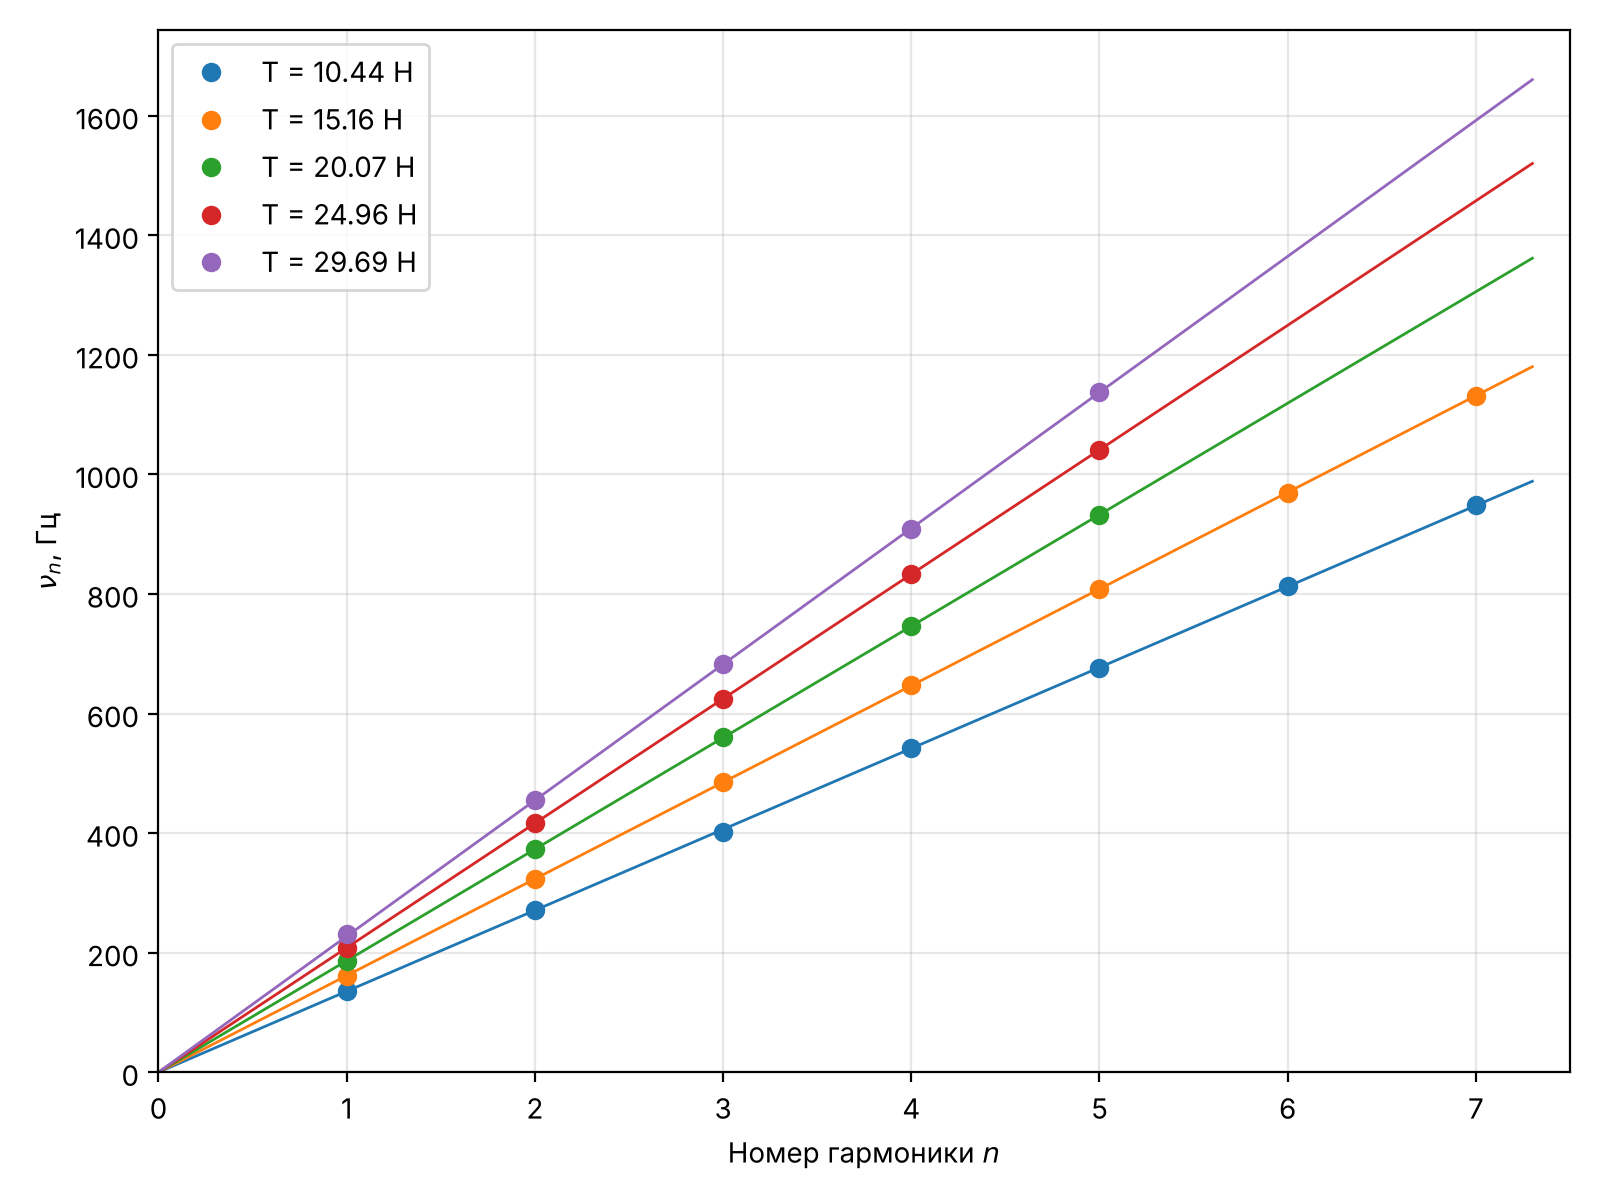
\includegraphics[width=0.85\textwidth]{nu_vs_n.png}
    \caption{Зависимость частоты от номера гармоники для различных натяжений}
    \label{fig:nun}
\end{figure}

Точки хорошо ложатся на прямые, проходящие через начало координат, то есть условие образования стоячих волн ($\nu_n\propto n$) выполняется. Коэффициент наклона $k=\nu_1$ найден по формуле $k=\sum n\nu_n/\sum n^2$, его погрешность $\sigma_k$ --- по разбросу точек относительно прямой. По наклону определена скорость волны $u=2Lk$, её погрешность
\begin{equation}
    \sigma_u = u\sqrt{\left(\frac{\sigma_L}{L}\right)^2+\left(\frac{\sigma_k}{k}\right)^2}.
\end{equation}

\begin{table}[H]
    \centering
    \caption{Скорости волн и их сравнение с теорией $u_{\text{теор}}=\sqrt{T/\rho_l^{\text{табл}}}$}
    \begin{tabular}{ccccc}
        \toprule
        $T$, Н & $k$, Гц & $u_{\text{эксп}}$, м/с & $u_{\text{теор}}$, м/с & отклонение, \% \\
        \midrule
        10,445 & $135{,}42\pm0{,}15$ & $135{,}4\pm0{,}3$ & 135,6 & $-0{,}1$ \\
        15,160 & $161{,}68\pm0{,}07$ & $161{,}7\pm0{,}3$ & 163,3 & $-1{,}0$ \\
        20,068 & $186{,}53\pm0{,}09$ & $186{,}5\pm0{,}4$ & 187,9 & $-0{,}7$ \\
        24,964 & $208{,}24\pm0{,}04$ & $208{,}2\pm0{,}4$ & 209,6 & $-0{,}6$ \\
        29,690 & $227{,}45\pm0{,}23$ & $227{,}5\pm0{,}5$ & 228,6 & $-0{,}5$ \\
        \bottomrule
    \end{tabular}
\end{table}

\subsection{Зависимость скорости от натяжения}

Из~\eqref{eq:u} следует $u^2=T/\rho_l$, то есть график $u^2(T)$ --- прямая, проходящая через начало координат, с наклоном $1/\rho_l$.

\begin{figure}[H]
    \centering
    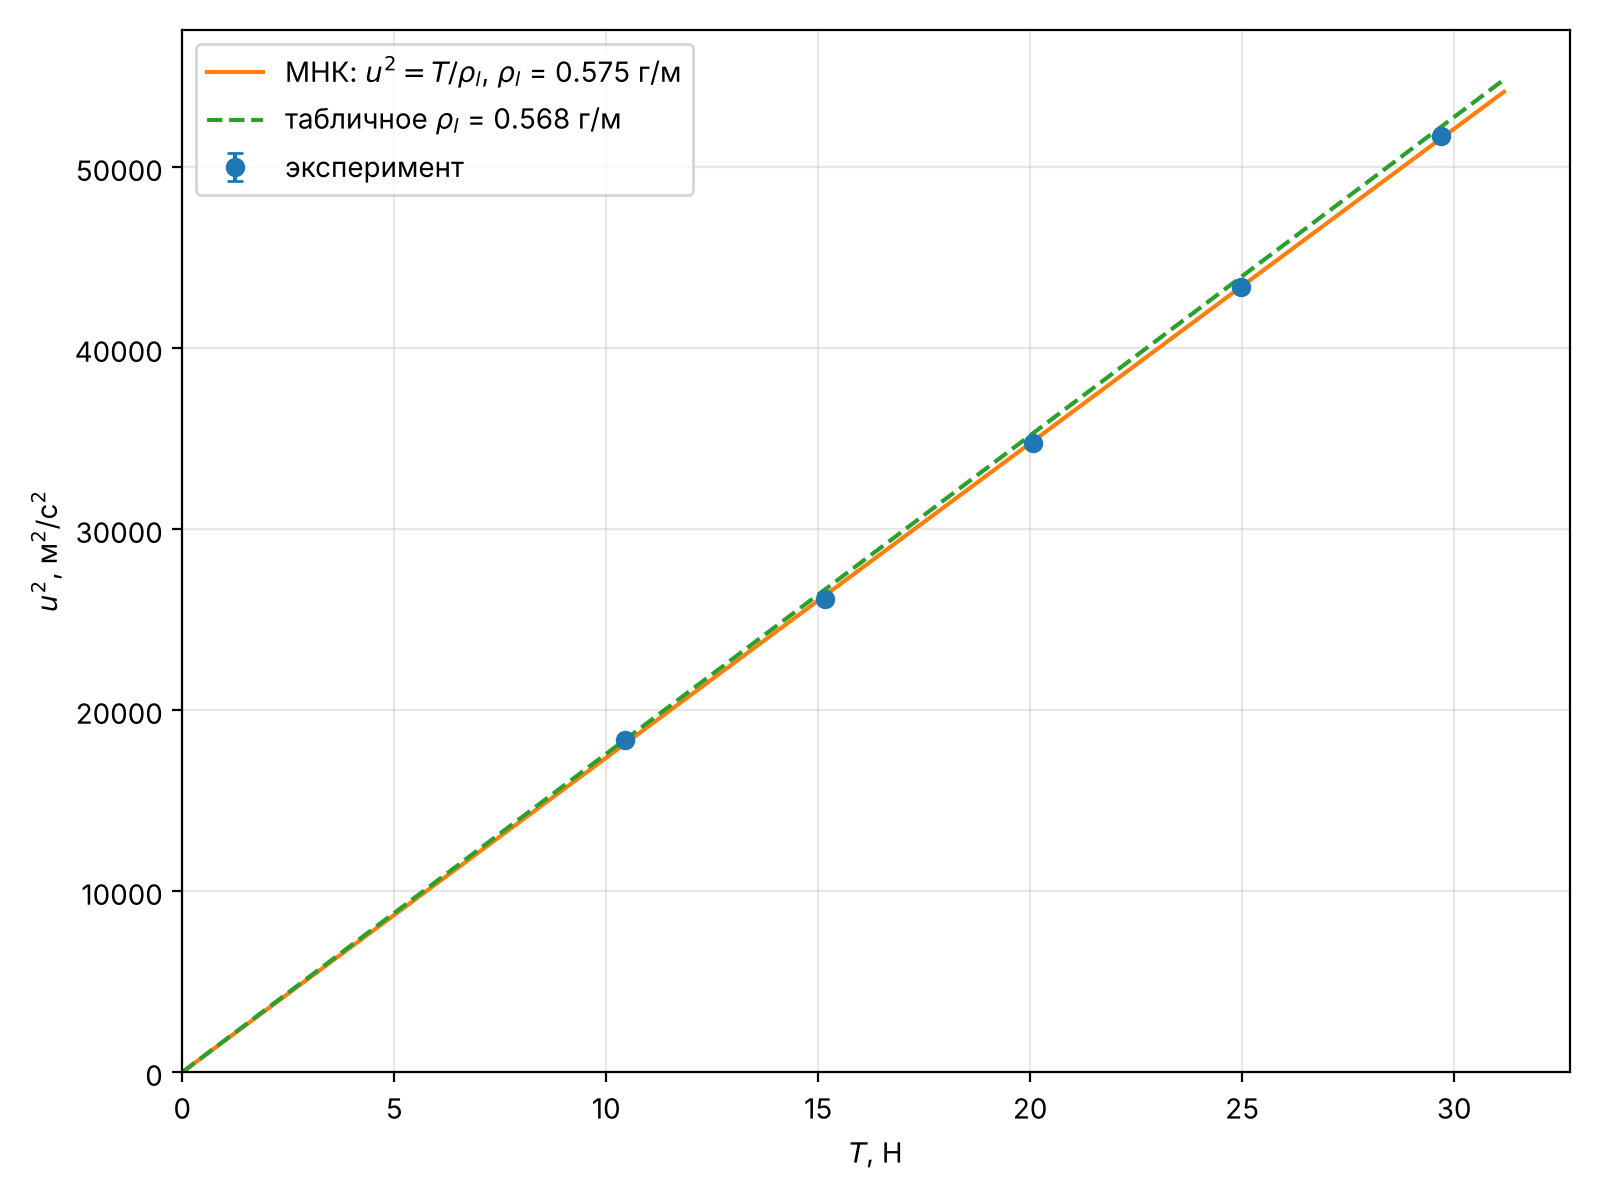
\includegraphics[width=0.85\textwidth]{u2_vs_T.png}
    \caption{Зависимость квадрата скорости от силы натяжения}
    \label{fig:u2T}
\end{figure}

Точки лежат на прямой, проходящей через начало координат. По методу наименьших квадратов (с учётом погрешностей $\sigma_{u^2}=2u\sigma_u$) получено $1/\rho_l=1737{,}6\pm3{,}3$~м/кг, откуда погонная плотность
\begin{equation}
    \rho_l^{\text{эксп}} = (575{,}5\pm2{,}5)\ \text{мг/м}.
\end{equation}
В погрешность включена систематическая составляющая от неточности измерения длины ($2\sigma_L/L=0{,}4\%$).

\section{Обсуждение результатов}

Полученное значение $\rho_l^{\text{эксп}}=(575{,}5\pm2{,}5)$~мг/м отличается от табличного $\rho_l^{\text{табл}}=568{,}4$~мг/м на $1{,}25\%$. Скорости, измеренные при четырёх натяжениях из пяти, оказываются на $0{,}5$--$1{,}0\%$ ниже теоретических, что и приводит к завышению $\rho_l$. Знак отклонения у них одинаков, поэтому оно является систематическим, а не случайным.

Возможные причины: трение в блоке, из-за которого реальное натяжение струны меньше $mg$; влияние зажима струны в стойке~3, который при затяжке может изменять натяжение и эффективную длину колеблющегося участка; погрешность определения резонанса (ширина резонансной кривой); небольшая бегущая компонента волны и нелинейные эффекты при большой амплитуде. Погрешность измерения длины струны даёт вклад лишь около $0{,}2\%$ в частоту и объяснить отклонение не может.

\section{Вывод}

В ходе работы были изучены стоячие волны на струне. Экспериментально подтверждено условие образования стоячих волн: частота резонанса пропорциональна номеру гармоники ($\nu_n\propto n$, графики --- прямые через начало координат). Проверена зависимость скорости поперечных волн от натяжения ($u^2\propto T$). Экспериментально определена погонная плотность струны $\rho_l=(575{,}5\pm2{,}5)$~мг/м, которая отличается от табличного значения $568{,}4$~мг/м на $1{,}25\%$.

\end{document}